
%% bare_jrnl_compsoc.tex
%% V1.3
%% 2007/01/11
%% by Michael Shell
%% See:
%% http://www.michaelshell.org/
%% for current contact information.
%%
%% This is a skeleton file demonstrating the use of IEEEtran.cls
%% (requires IEEEtran.cls version 1.7 or later) with an IEEE Computer
%% Society journal paper.
%%
%% Support sites:
%% http://www.michaelshell.org/tex/ieeetran/
%% http://www.ctan.org/tex-archive/macros/latex/contrib/IEEEtran/
%% and
%% http://www.ieee.org/

%%*************************************************************************
%% Legal Notice:
%% This code is offered as-is without any warranty either expressed or
%% implied; without even the implied warranty of MERCHANTABILITY or
%% FITNESS FOR A PARTICULAR PURPOSE!
%% User assumes all risk.
%% In no event shall IEEE or any contributor to this code be liable for
%% any damages or losses, including, but not limited to, incidental,
%% consequential, or any other damages, resulting from the use or misuse
%% of any information contained here.
%%
%% All comments are the opinions of their respective authors and are not
%% necessarily endorsed by the IEEE.
%%
%% This work is distributed under the LaTeX Project Public License (LPPL)
%% ( http://www.latex-project.org/ ) version 1.3, and may be freely used,
%% distributed and modified. A copy of the LPPL, version 1.3, is included
%% in the base LaTeX documentation of all distributions of LaTeX released
%% 2003/12/01 or later.
%% Retain all contribution notices and credits.
%% ** Modified files should be clearly indicated as such, including  **
%% ** renaming them and changing author support contact information. **
%%
%% File list of work: IEEEtran.cls, IEEEtran_HOWTO.pdf, bare_adv.tex,
%%                    bare_conf.tex, bare_jrnl.tex, bare_jrnl_compsoc.tex
%%*************************************************************************

% *** Authors should verify (and, if needed, correct) their LaTeX system  ***
% *** with the testflow diagnostic prior to trusting their LaTeX platform ***
% *** with production work. IEEE's font choices can trigger bugs that do  ***
% *** not appear when using other class files.                            ***
% The testflow support page is at:
% http://www.michaelshell.org/tex/testflow/




% Note that the a4paper option is mainly intended so that authors in
% countries using A4 can easily print to A4 and see how their papers will
% look in print - the typesetting of the document will not typically be
% affected with changes in paper size (but the bottom and side margins will).
% Use the testflow package mentioned above to verify correct handling of
% both paper sizes by the user's LaTeX system.
%
% Also note that the "draftcls" or "draftclsnofoot", not "draft", option
% should be used if it is desired that the figures are to be displayed in
% draft mode.
%
% The Computer Society usually requires 12pt for submissions.
%
\documentclass[12pt,journal,compsoc]{IEEEtran}
%
% If IEEEtran.cls has not been installed into the LaTeX system files,
% manually specify the path to it like:
% \documentclass[12pt,journal,compsoc]{../sty/IEEEtran}






% Some very useful LaTeX packages include:
% (uncomment the ones you want to load)


% *** MISC UTILITY PACKAGES ***
%
%\usepackage{ifpdf}
% Heiko Oberdiek's ifpdf.sty is very useful if you need conditional
% compilation based on whether the output is pdf or dvi.
% usage:
% \ifpdf
%   % pdf code
% \else
%   % dvi code
% \fi
% The latest version of ifpdf.sty can be obtained from:
% http://www.ctan.org/tex-archive/macros/latex/contrib/oberdiek/
% Also, note that IEEEtran.cls V1.7 and later provides a builtin
% \ifCLASSINFOpdf conditional that works the same way.
% When switching from latex to pdflatex and vice-versa, the compiler may
% have to be run twice to clear warning/error messages.






% *** CITATION PACKAGES ***
%
\ifCLASSOPTIONcompsoc
  % IEEE Computer Society needs nocompress option
  % requires cite.sty v4.0 or later (November 2003)
   \usepackage[nocompress]{cite}
\else
  % normal IEEE
   \usepackage{cite}
\fi
% cite.sty was written by Donald Arseneau
% V1.6 and later of IEEEtran pre-defines the format of the cite.sty package
% \cite{} output to follow that of IEEE. Loading the cite package will
% result in citation numbers being automatically sorted and properly
% "compressed/ranged". e.g., [1], [9], [2], [7], [5], [6] without using
% cite.sty will become [1], [2], [5]--[7], [9] using cite.sty. cite.sty's
% \cite will automatically add leading space, if needed. Use cite.sty's
% noadjust option (cite.sty V3.8 and later) if you want to turn this off.
% cite.sty is already installed on most LaTeX systems. Be sure and use
% version 4.0 (2003-05-27) and later if using hyperref.sty. cite.sty does
% not currently provide for hyperlinked citations.
% The latest version can be obtained at:
% http://www.ctan.org/tex-archive/macros/latex/contrib/cite/
% The documentation is contained in the cite.sty file itself.
%
% Note that some packages require special options to format as the Computer
% Society requires. In particular, Computer Society  papers do not use
% compressed citation ranges as is done in typical IEEE papers
% (e.g., [1]-[4]). Instead, they list every citation separately in order
% (e.g., [1], [2], [3], [4]). To get the latter we need to load the cite
% package with the nocompress option which is supported by cite.sty v4.0
% and later. Note also the use of a CLASSOPTION conditional provided by
% IEEEtran.cls V1.7 and later.





% *** GRAPHICS RELATED PACKAGES ***
%
\ifCLASSINFOpdf
   \usepackage[pdftex]{graphicx}
  % declare the path(s) where your graphic files are
   \graphicspath{{./pdf/}{./jpeg/}}
  % and their extensions so you won't have to specify these with
  % every instance of \includegraphics
   \DeclareGraphicsExtensions{.pdf,.jpeg,.png}
\else
  % or other class option (dvipsone, dvipdf, if not using dvips). graphicx
  % will default to the driver specified in the system graphics.cfg if no
  % driver is specified.
   \usepackage[dvips]{graphicx}
  % declare the path(s) where your graphic files are
   \graphicspath{{./eps/}}
  % and their extensions so you won't have to specify these with
  % every instance of \includegraphics
   \DeclareGraphicsExtensions{.eps}
\fi
% graphicx was written by David Carlisle and Sebastian Rahtz. It is
% required if you want graphics, photos, etc. graphicx.sty is already
% installed on most LaTeX systems. The latest version and documentation can
% be obtained at:
% http://www.ctan.org/tex-archive/macros/latex/required/graphics/
% Another good source of documentation is "Using Imported Graphics in
% LaTeX2e" by Keith Reckdahl which can be found as epslatex.ps or
% epslatex.pdf at: http://www.ctan.org/tex-archive/info/
%
% latex, and pdflatex in dvi mode, support graphics in encapsulated
% postscript (.eps) format. pdflatex in pdf mode supports graphics
% in .pdf, .jpeg, .png and .mps (metapost) formats. Users should ensure
% that all non-photo figures use a vector format (.eps, .pdf, .mps) and
% not a bitmapped formats (.jpeg, .png). IEEE frowns on bitmapped formats
% which can result in "jaggedy"/blurry rendering of lines and letters as
% well as large increases in file sizes.
%
% You can find documentation about the pdfTeX application at:
% http://www.tug.org/applications/pdftex





% *** MATH PACKAGES ***
%
\usepackage[cmex10]{amsmath}
% A popular package from the American Mathematical Society that provides
% many useful and powerful commands for dealing with mathematics. If using
% it, be sure to load this package with the cmex10 option to ensure that
% only type 1 fonts will utilized at all point sizes. Without this option,
% it is possible that some math symbols, particularly those within
% footnotes, will be rendered in bitmap form which will result in a
% document that can not be IEEE Xplore compliant!
%
% Also, note that the amsmath package sets \interdisplaylinepenalty to 10000
% thus preventing page breaks from occurring within multiline equations. Use:
\interdisplaylinepenalty=2500
% after loading amsmath to restore such page breaks as IEEEtran.cls normally
% does. amsmath.sty is already installed on most LaTeX systems. The latest
% version and documentation can be obtained at:
% http://www.ctan.org/tex-archive/macros/latex/required/amslatex/math/





% *** SPECIALIZED LIST PACKAGES ***
%
\usepackage{algorithmic}
% algorithmic.sty was written by Peter Williams and Rogerio Brito.
% This package provides an algorithmic environment for describing algorithms.
% You can use the algorithmic environment in-text or within a figure
% environment to provide for a floating algorithm. Do NOT use the algorithm
% floating environment provided by algorithm.sty (by the same authors) or
% algorithm2e.sty (by Christophe Fiorio) as IEEE does not use dedicated
% algorithm float types and packages that provide these will not provide
% correct IEEE style captions. The latest version and documentation of
% algorithmic.sty can be obtained at:
% http://www.ctan.org/tex-archive/macros/latex/contrib/algorithms/
% There is also a support site at:
% http://algorithms.berlios.de/index.html
% Also of interest may be the (relatively newer and more customizable)
% algorithmicx.sty package by Szasz Janos:
% http://www.ctan.org/tex-archive/macros/latex/contrib/algorithmicx/




% *** ALIGNMENT PACKAGES ***
%
\usepackage{array}
% Frank Mittelbach's and David Carlisle's array.sty patches and improves
% the standard LaTeX2e array and tabular environments to provide better
% appearance and additional user controls. As the default LaTeX2e table
% generation code is lacking to the point of almost being broken with
% respect to the quality of the end results, all users are strongly
% advised to use an enhanced (at the very least that provided by array.sty)
% set of table tools. array.sty is already installed on most systems. The
% latest version and documentation can be obtained at:
% http://www.ctan.org/tex-archive/macros/latex/required/tools/


\usepackage{mdwmath}
\usepackage{mdwtab}
% Also highly recommended is Mark Wooding's extremely powerful MDW tools,
% especially mdwmath.sty and mdwtab.sty which are used to format equations
% and tables, respectively. The MDWtools set is already installed on most
% LaTeX systems. The lastest version and documentation is available at:
% http://www.ctan.org/tex-archive/macros/latex/contrib/mdwtools/


% IEEEtran contains the IEEEeqnarray family of commands that can be used to
% generate multiline equations as well as matrices, tables, etc., of high
% quality.


\usepackage{eqparbox}
% Also of notable interest is Scott Pakin's eqparbox package for creating
% (automatically sized) equal width boxes - aka "natural width parboxes".
% Available at:
% http://www.ctan.org/tex-archive/macros/latex/contrib/eqparbox/





% *** SUBFIGURE PACKAGES ***
%\ifCLASSOPTIONcompsoc
%\usepackage[tight,normalsize,sf,SF]{subfigure}
%\else
%\usepackage[tight,footnotesize]{subfigure}
%\fi
% subfigure.sty was written by Steven Douglas Cochran. This package makes it
% easy to put subfigures in your figures. e.g., "Figure 1a and 1b". For IEEE
% work, it is a good idea to load it with the tight package option to reduce
% the amount of white space around the subfigures. Computer Society papers
% use a larger font and \sffamily font for their captions, hence the
% additional options needed under compsoc mode. subfigure.sty is already
% installed on most LaTeX systems. The latest version and documentation can
% be obtained at:
% http://www.ctan.org/tex-archive/obsolete/macros/latex/contrib/subfigure/
% subfigure.sty has been superceeded by subfig.sty.


%\ifCLASSOPTIONcompsoc
%  \usepackage[caption=false]{caption}
%  \usepackage[font=normalsize,labelfont=sf,textfont=sf]{subfig}
%\else
%  \usepackage[caption=false]{caption}
%  \usepackage[font=footnotesize]{subfig}
%\fi
% subfig.sty, also written by Steven Douglas Cochran, is the modern
% replacement for subfigure.sty. However, subfig.sty requires and
% automatically loads Axel Sommerfeldt's caption.sty which will override
% IEEEtran.cls handling of captions and this will result in nonIEEE style
% figure/table captions. To prevent this problem, be sure and preload
% caption.sty with its "caption=false" package option. This is will preserve
% IEEEtran.cls handing of captions. Version 1.3 (2005/06/28) and later
% (recommended due to many improvements over 1.2) of subfig.sty supports
% the caption=false option directly:
\ifCLASSOPTIONcompsoc
  \usepackage[caption=false,font=normalsize,labelfont=sf,textfont=sf]{subfig}
\else
  \usepackage[caption=false,font=footnotesize]{subfig}
\fi
%
% The latest version and documentation can be obtained at:
% http://www.ctan.org/tex-archive/macros/latex/contrib/subfig/
% The latest version and documentation of caption.sty can be obtained at:
% http://www.ctan.org/tex-archive/macros/latex/contrib/caption/




% *** FLOAT PACKAGES ***
%
\usepackage{fixltx2e}
% fixltx2e, the successor to the earlier fix2col.sty, was written by
% Frank Mittelbach and David Carlisle. This package corrects a few problems
% in the LaTeX2e kernel, the most notable of which is that in current
% LaTeX2e releases, the ordering of single and double column floats is not
% guaranteed to be preserved. Thus, an unpatched LaTeX2e can allow a
% single column figure to be placed prior to an earlier double column
% figure. The latest version and documentation can be found at:
% http://www.ctan.org/tex-archive/macros/latex/base/



\usepackage{stfloats}
% stfloats.sty was written by Sigitas Tolusis. This package gives LaTeX2e
% the ability to do double column floats at the bottom of the page as well
% as the top. (e.g., "\begin{figure*}[!b]" is not normally possible in
% LaTeX2e). It also provides a command:
\fnbelowfloat
% to enable the placement of footnotes below bottom floats (the standard
% LaTeX2e kernel puts them above bottom floats). This is an invasive package
% which rewrites many portions of the LaTeX2e float routines. It may not work
% with other packages that modify the LaTeX2e float routines. The latest
% version and documentation can be obtained at:
% http://www.ctan.org/tex-archive/macros/latex/contrib/sttools/
% Documentation is contained in the stfloats.sty comments as well as in the
% presfull.pdf file. Do not use the stfloats baselinefloat ability as IEEE
% does not allow \baselineskip to stretch. Authors submitting work to the
% IEEE should note that IEEE rarely uses double column equations and
% that authors should try to avoid such use. Do not be tempted to use the
% cuted.sty or midfloat.sty packages (also by Sigitas Tolusis) as IEEE does
% not format its papers in such ways.




%\ifCLASSOPTIONcaptionsoff
%  \usepackage[nomarkers]{endfloat}
% \let\MYoriglatexcaption\caption
% \renewcommand{\caption}[2][\relax]{\MYoriglatexcaption[#2]{#2}}
%\fi
% endfloat.sty was written by James Darrell McCauley and Jeff Goldberg.
% This package may be useful when used in conjunction with IEEEtran.cls'
% captionsoff option. Some IEEE journals/societies require that submissions
% have lists of figures/tables at the end of the paper and that
% figures/tables without any captions are placed on a page by themselves at
% the end of the document. If needed, the draftcls IEEEtran class option or
% \CLASSINPUTbaselinestretch interface can be used to increase the line
% spacing as well. Be sure and use the nomarkers option of endfloat to
% prevent endfloat from "marking" where the figures would have been placed
% in the text. The two hack lines of code above are a slight modification of
% that suggested by in the endfloat docs (section 8.3.1) to ensure that
% the full captions always appear in the list of figures/tables - even if
% the user used the short optional argument of \caption[]{}.
% IEEE papers do not typically make use of \caption[]'s optional argument,
% so this should not be an issue. A similar trick can be used to disable
% captions of packages such as subfig.sty that lack options to turn off
% the subcaptions:
% For subfig.sty:
% \let\MYorigsubfloat\subfloat
% \renewcommand{\subfloat}[2][\relax]{\MYorigsubfloat[]{#2}}
% For subfigure.sty:
% \let\MYorigsubfigure\subfigure
% \renewcommand{\subfigure}[2][\relax]{\MYorigsubfigure[]{#2}}
% However, the above trick will not work if both optional arguments of
% the \subfloat/subfig command are used. Furthermore, there needs to be a
% description of each subfigure *somewhere* and endfloat does not add
% subfigure captions to its list of figures. Thus, the best approach is to
% avoid the use of subfigure captions (many IEEE journals avoid them anyway)
% and instead reference/explain all the subfigures within the main caption.
% The latest version of endfloat.sty and its documentation can obtained at:
% http://www.ctan.org/tex-archive/macros/latex/contrib/endfloat/
%
% The IEEEtran \ifCLASSOPTIONcaptionsoff conditional can also be used
% later in the document, say, to conditionally put the References on a
% page by themselves.




% *** PDF, URL AND HYPERLINK PACKAGES ***
%
\usepackage{url}
% url.sty was written by Donald Arseneau. It provides better support for
% handling and breaking URLs. url.sty is already installed on most LaTeX
% systems. The latest version can be obtained at:
% http://www.ctan.org/tex-archive/macros/latex/contrib/misc/
% Read the url.sty source comments for usage information. Basically,
% \url{my_url_here}.



% \newtheorem sets are defined here
\newtheorem{definition}{Definition}




% *** Do not adjust lengths that control margins, column widths, etc. ***
% *** Do not use packages that alter fonts (such as pslatex).         ***
% There should be no need to do such things with IEEEtran.cls V1.6 and later.
% (Unless specifically asked to do so by the journal or conference you plan
% to submit to, of course. )

% I still do not think hyperref is a bad package.
\usepackage{hyperref}
\hypersetup{unicode}
\hypersetup{colorlinks=true}
\hypersetup{linkcolor=black}


% correct bad hyphenation here
\hyphenation{op-tical net-works semi-conduc-tor}


\begin{document}
%
% paper title
% can use linebreaks \\ within to get better formatting as desired
%\title{Bare Demo of IEEEtran.cls\\ for Computer Society Journals}
\title{RSA and El-Gamal Cryptosystems}
%
%
% author names and IEEE memberships
% note positions of commas and nonbreaking spaces ( ~ ) LaTeX will not break
% a structure at a ~ so this keeps an author's name from being broken across
% two lines.
% use \thanks{} to gain access to the first footnote area
% a separate \thanks must be used for each paragraph as LaTeX2e's \thanks
% was not built to handle multiple paragraphs
%
%
%\IEEEcompsocitemizethanks is a special \thanks that produces the bulleted
% lists the Computer Society journals use for "first footnote" author
% affiliations. Use \IEEEcompsocthanksitem which works much like \item
% for each affiliation group. When not in compsoc mode,
% \IEEEcompsocitemizethanks becomes like \thanks and
% \IEEEcompsocthanksitem becomes a line break with idention. This
% facilitates dual compilation, although admittedly the differences in the
% desired content of \author between the different types of papers makes a
% one-size-fits-all approach a daunting prospect. For instance, compsoc
% journal papers have the author affiliations above the "Manuscript
% received ..."  text while in non-compsoc journals this is reversed. Sigh.

%\author{Michael~Shell,~\IEEEmembership{Member,~IEEE,}
%        John~Doe,~\IEEEmembership{Fellow,~OSA,}
%        and~Jane~Doe,~\IEEEmembership{Life~Fellow,~IEEE}% <-this % stops a space
%\IEEEcompsocitemizethanks{\IEEEcompsocthanksitem M. Shell is with the Department
%of Electrical and Computer Engineering, Georgia Institute of Technology, Atlanta,
%GA, 30332.\protect\\
% note need leading \protect in front of \\ to get a newline within \thanks as
% \\ is fragile and will error, could use \hfil\break instead.
%E-mail: see http://www.michaelshell.org/contact.html
%\IEEEcompsocthanksitem J. Doe and J. Doe are with Anonymous University.}% <-this % stops a space
%\thanks{Manuscript received April 19, 2005; revised January 11, 2007.}}
\author{Yanan~Xiao,~\IEEEmembership{Student~Member,~IEEE}
Maryam~Al~Mehrezi%
\IEEEcompsocitemizethanks{\IEEEcompsocthanksitem Yanan Xiao and Maryam
  Al Mehrezi are with the Department of Electrical Engineering and
Computer Science, Masdar Institute of Science and Technology, Masdar City,
Abu Dhabi, UAE, 54224.\protect\\
E-mail: \{yxiao,malmehrezi\}@masdar.ac.ae}}

% note the % following the last \IEEEmembership and also \thanks -
% these prevent an unwanted space from occurring between the last author name
% and the end of the author line. i.e., if you had this:
%
% \author{....lastname \thanks{...} \thanks{...} }
%                     ^------------^------------^----Do not want these spaces!
%
% a space would be appended to the last name and could cause every name on that
% line to be shifted left slightly. This is one of those "LaTeX things". For
% instance, "\textbf{A} \textbf{B}" will typeset as "A B" not "AB". To get
% "AB" then you have to do: "\textbf{A}\textbf{B}"
% \thanks is no different in this regard, so shield the last } of each \thanks
% that ends a line with a % and do not let a space in before the next \thanks.
% Spaces after \IEEEmembership other than the last one are OK (and needed) as
% you are supposed to have spaces between the names. For what it is worth,
% this is a minor point as most people would not even notice if the said evil
% space somehow managed to creep in.



% The paper headers
\markboth{Journal of Masdar Institute,~Vol.~16, No.~1, October~2013}%
{RSA and El-Gamal Cryptosystems}
% The only time the second header will appear is for the odd numbered pages
% after the title page when using the twoside option.
%
% *** Note that you probably will NOT want to include the author's ***
% *** name in the headers of peer review papers.                   ***
% You can use \ifCLASSOPTIONpeerreview for conditional compilation here if
% you desire.



% The publisher's ID mark at the bottom of the page is less important with
% Computer Society journal papers as those publications place the marks
% outside of the main text columns and, therefore, unlike regular IEEE
% journals, the available text space is not reduced by their presence.
% If you want to put a publisher's ID mark on the page you can do it like
% this:
%\IEEEpubid{0000--0000/00\$00.00~\copyright~2007 IEEE}
% or like this to get the Computer Society new two part style.
%\IEEEpubid{\makebox[\columnwidth]{\hfill 0000--0000/00/\$00.00~\copyright~2007 IEEE}%
%\hspace{\columnsep}\makebox[\columnwidth]{Published by the IEEE Computer Society\hfill}}
% Remember, if you use this you must call \IEEEpubidadjcol in the second
% column for its text to clear the IEEEpubid mark (Computer Society jorunal
% papers don't need this extra clearance.)



% use for special paper notices
%\IEEEspecialpapernotice{(Invited Paper)}



% for Computer Society papers, we must declare the abstract and index terms
% PRIOR to the title within the \IEEEcompsoctitleabstractindextext IEEEtran
% command as these need to go into the title area created by \maketitle.
\IEEEcompsoctitleabstractindextext{%
\begin{abstract}
%\boldmath
We present our analysis of RSA and ElGamal cryptosystem with great
detail. We show that there are some attacks on RSA.\@ The mathematical
foundation of ElGamal cryptosystem, namely discrete logarithm problem
is discussed. Basic structure of our implementation codes is also mentioned.
\end{abstract}
% IEEEtran.cls defaults to using nonbold math in the Abstract.
% This preserves the distinction between vectors and scalars. However,
% if the journal you are submitting to favors bold math in the abstract,
% then you can use LaTeX's standard command \boldmath at the very start
% of the abstract to achieve this. Many IEEE journals frown on math
% in the abstract anyway. In particular, the Computer Society does
% not want either math or citations to appear in the abstract.

% Note that keywords are not normally used for peerreview papers.
\begin{IEEEkeywords}
RSA, El-Gamal, implementation, public key, cryptosystem
\end{IEEEkeywords}}


% make the title area
\maketitle


% To allow for easy dual compilation without having to reenter the
% abstract/keywords data, the \IEEEcompsoctitleabstractindextext text will
% not be used in maketitle, but will appear (i.e., to be "transported")
% here as \IEEEdisplaynotcompsoctitleabstractindextext when compsoc mode
% is not selected <OR> if conference mode is selected - because compsoc
% conference papers position the abstract like regular (non-compsoc)
% papers do!
\IEEEdisplaynotcompsoctitleabstractindextext%
% \IEEEdisplaynotcompsoctitleabstractindextext has no effect when using
% compsoc under a non-conference mode.


% For peer review papers, you can put extra information on the cover
% page as needed:
% \ifCLASSOPTIONpeerreview
% \begin{center} \bfseries EDICS Category: 3-BBND \end{center}
% \fi
%
% For peerreview papers, this IEEEtran command inserts a page break and
% creates the second title. It will be ignored for other modes.
\IEEEpeerreviewmaketitle%



\section{Introduction}
\label{sec:introduction}
% Computer Society journal papers do something a tad strange with the very
% first section heading (almost always called "Introduction"). They place it
% ABOVE the main text! IEEEtran.cls currently does not do this for you.
% However, You can achieve this effect by making LaTeX jump through some
% hoops via something like:
%
%\ifCLASSOPTIONcompsoc
%  \noindent\raisebox{2\baselineskip}[0pt][0pt]%
%  {\parbox{\columnwidth}{\section{Introduction}\label{sec:introduction}%
%  \global\everypar=\everypar}}%
%  \vspace{-1\baselineskip}\vspace{-\parskip}\par
%\else
%  \section{Introduction}\label{sec:introduction}\par
%\fi
%
% Admittedly, this is a hack and may well be fragile, but seems to do the
% trick for me. Note the need to keep any \label that may be used right
% after \section in the above as the hack puts \section within a raised box.



% The very first letter is a 2 line initial drop letter followed
% by the rest of the first word in caps (small caps for compsoc).
%
% form to use if the first word consists of a single letter:
% \IEEEPARstart{A}{demo} file is ....
%
% form to use if you need the single drop letter followed by
% normal text (unknown if ever used by IEEE):
% \IEEEPARstart{A}{}demo file is ....
%
% Some journals put the first two words in caps:
% \IEEEPARstart{T}{his demo} file is ....
%
% Here we have the typical use of a "T" for an initial drop letter
% and "HIS" in caps to complete the first word.
% \IEEEPARstart{T}{his} demo file is intended to serve as a ``starter file''
% for IEEE Computer Society journal papers produced under \LaTeX\ using
% IEEEtran.cls version 1.7 and later.
% % You must have at least 2 lines in the paragraph with the drop letter
% % (should never be an issue)
% I wish you the best of success.
\IEEEPARstart{C}{ryptography}  is a fascinating subject. The spread of
computers and communication systems require private sector to protect
the information in digital form, and to provide security
services. Further, Cryptography has a great importance in most
technology today, not only in computers but also in credit cards,
government and it remains the standard means for securing electronic
commerce for many financial institutions around the world. 
\par
Cryptography is the science of encoding data, typically using a key,
so that people without the key cannot read the data. Many different
algorithms are used to encrypt data and they are either symmetric or
asymmetric. In symmetric key cryptography, the best known algorithm is
the Data Encryption Standard (DES). DES, which was developed at IBM in
1977, was a popular standers algorithm for years, until Triple DES and
AES began to replace it. Whereas, symmetric key algorithms require a
shared secret to be exchanged between the communicating parties to
have a secured communication
see~\autoref{fig:intro-process-of-symmetric}. 
\begin{figure}[!t]
  \centering
  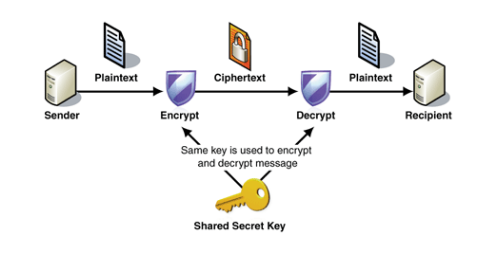
\includegraphics[scale=0.5]{Figure/Symmetric}
  \caption{The process of symmetric encryption}
  \label{fig:intro-process-of-symmetric}
\end{figure}
The security of the symmetric key algorithm depends on the secrecy of
the key. So, the problem with symmetric keys is how to securely get
the secret keys to each end of the exchange and keep them secure after
that. For this reason, an asymmetric key system is now often used that
is known as the public key infrastructure (PKI). Public-key encryption
does not require that you openly exchange a secret key with the
recipient of an encrypted message. 
\par
Public-key cryptography also referred to as asymmetric encryption,
uses a pair of cryptographic keys, a public key and a private key see 
\begin{figure}[!t]
  \centering
  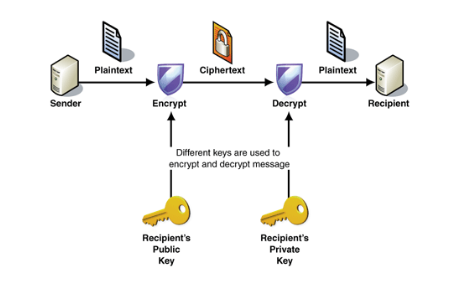
\includegraphics[scale=0.5]{Figure/Asymmetric.png}
  \caption{The process of asymmetric encryption}
  \label{fig:intro-process-of-asymetric}
\end{figure} 
The private key is kept secret and defines the associated
decryption transformation, while the public key defines an encryption
transformation and can be distributed openly, thereby negating the
need to transmit a secret key in advance. The keys are related
mathematically, allowing the sender of a message to encrypt his
message using the recipient's public key. The message can then only be
decrypted using the recipient's private key. Since encryption
transformation is public knowledge, public-key encryption alone does
not provide data origin authentication or data integrity. Public-key
decryption by using private key can provides authentication guarantees
in entity authentication and authenticated key establishment
protocols. So, public-key encryption provides both privacy and
confidentiality. 
\par
Public-key encryption schemes are simple, elegant and relatively
efficient digital signature mechanisms. The key used to describe the
public verification function is typically much smaller than for the
symmetric-key counterpart. However they are typically substantially
slower than symmetric-key encryption algorithms. For this reason,
public-key encryption is most commonly used in practice for the
transport of keys subsequently used for bulk data encryption by
symmetric algorithms and other applications including data integrity
and authentication, and for encrypting small data items such as credit
card numbers and PINs.
\par
Public-key cryptography being discovered in the mid-1970s and it does
not have an extensive history as symmetric-key encryption, but the
most familiar public-key algorithms are RSA and Diffie–Hellman key
exchange, while the Digital Signature Algorithm is the most widely
used digital signature system. 
\par
There are several public key algorithms. The first one proposed is the
knapsack cryptosystem but it is insecure and an easily understood
system. After the knapsack, RSA algorithm is known as the gold
standard of public key cryptography that we will focus on it in this
report. Then, The Diffie–Hellman key exchange was published in 1976 by
Whitfield Diffie and MartinHellman and it provided a common secret key
between the communicating parties over an insecure channel. 
\par
Also there are more public key algorithms such as El-Gamal
Cryptosystem and Elliptic Curve Cryptosystem (ECC), but in this report
we are mainly focused on some asymmetric algorithms which are mostly
used. They are RSA and ElGamal cryptosystems.  



% \hfill mds

% \hfill January 11, 2007

% \subsection{Subsection Heading Here}
% Subsection text here.


% needed in second column of first page if using \IEEEpubid
%\IEEEpubidadjcol

%\subsubsection{Subsubsection Heading Here}
%Subsubsection text here.

%\section{Related Work}
%Some related work will be discussed here.

% \section{Public Key Cryptosystem}
% \label{sec:publ-key-crypt}

% \subsection{More Details}

% Some problems with this template...I mean, the subsubsection part.

\section{RSA Cryptosystem}
\label{sec:rsa-cryptosystem}


RSA algorithm is used for public key cryptography and digital
signatures. It is the most commonly used public key encryption
algorithm. The security of the RSA algorithm is based on the
difficulty of factoring large numbers n = pq, where p and q are large
prime numbers. The RSA algorithm keys are often of length a power of
two, like 512, 1024, or 2048 bits, RSA to be secure, the key length
has to be at least 1024-bits. 
\par
This section will provide the history of RSA, describes the RSA
encryption scheme, its security, and provides some Practical
Considerations. 
\par

\subsection{RSA Background}
\label{sec:rsa-background}

RSA invented by Rivest, Shamir and Adleman in 1977, RSA stands for the
first letter in each of its inventors' last names. It was first
published in the paper A Method for Obtaining Digital Signatures and
Public-Key Cryptosystems, but the National Security Agency (NSA) did
not like the idea of the distribution the cryptography source code
internationally, and requested to be stopped. However, they continued
distribution because the NSA failed to provide a legal basis for their
request.  
\par

\subsection{RSA Details}
\label{sec:rsa-details}


RSA system involves three steps: key generation, encryption and
decryption. First step: key generation, the mathematical details of
the algorithm used in obtaining the public and private keys are
explained as follows:
\begin{enumerate}
\item Take two large primes, p and q, and compute their product n =
  pq, where n is called the modulus. 
\item Choose a number, e which is less than n and relatively prime to
  $(p-1)(q-1)$, that means e and (p-1)(q-1) have no common  factors
  except 1. 
\item Find another number d such that $(ed - 1)$ is divisible by
  $(p-1)(q-1)$. Whereas the values e and d are called the public and
  private exponents, respectively. 
\end{enumerate}
\par
The public key is the pair (n, e); the private key is (n, d). The
factors p and q may be destroyed or kept with the private key. 
\par
It is currently difficult to obtain the private key d from the public
key (n, e). However if one could factor n into p and q, then one could
obtain the private key d. Thus the security of the RSA system is based
on the assumption that factoring is difficult. The discovery of an
easy method of factoring would ``break'' RSA. 
\par
Second step: encryption, the ciphertext C is found by the equation $C
= M^{e}\mod n$ where M is the original message and e is the public or
encryption exponent. 
\par
Third step: decryption, the message M can be found form the ciphertext
C by the equation $M = C^{d}\mod n$ where d is the private or decryption
exponent. 
\par
The RSA system can be used for public key cryptography (encryption)
and digital signatures as we said before, there is slightly different
between them. 
\par
In RSA, encryption keys are public, while the decryption keys are
private, so no one can decrypt an encrypted message except the person
who has the private key. Everyone has their own public and private
keys. The keys must be made in such a way that the private key may not
be easily construed from the public encryption key. 

\subsection{Known Attacks on RSA Cryptosystem}
\label{sec:known-attacks-rsa}

The RSA function is a one-way trapdoor function. It is not known to be
easily invertible without the trapdoor, d. General attacks on RSA
involve trying to compute d, or some other way to get to M
(plaintext). The difficulties and the main security of RSA algorithm
is based on prime factorization problem. 
\par
There has been much research and many publications on attacks on the
RSA Cryptosystem.  We can categorize attacks on RSA into five
categories as below, and we will present a summary of them.

\subsubsection{\qquad Factoring large integers}
\label{sec:qquad-fact-large}

Given (C, e, N), Marvin can do a brute force search to find M. But
factoring N involves a much smaller search space and thus, more
efficient to do. Factoring is a well-researched
problem. Pomerance~\cite{pomerance2008tale} has an interesting
introduction into what clever methods can be done.  For example, how
to factor 8051?  Naive approach is trying all primes up to square root
of 8051, or almost 90.  Clever trick is to find a square of primes
that subtract to the number, i.e.$ 90^{2} – 7^{2} = 8051$. Thus $(90 –
7) * (90 + 7) = 8051$, $83$ and $97$ are the factors. However, this
trick is only easy if factors are close to square root of the number.
There are only a very small set of numbers where this is true.  But
much more sophisticated methods are known.  Currently the general
number field sieve is the best known running time with, reported by
Boneh~\cite{boneh1999twenty}, a time on n-bit integers of
$\exp^{(c+o(1))n^{1/3}\log^{2/3}n}$ for some $c<2$.
\par
To be complete, Peter Shor~\cite{Shor:1994jg} has shown a
quantum computer has a polynomial time algorithm for factoring
integers. But engineering a quantum computer still has a way to go, so
RSA is safe for now. 
\par
RSA security depends on the computation to be unreasonable for 1) the
factoring of N, and 2) computing the e\emph{th} roots modulo N. The first is
fairly well researched and complexity is understood. However, the
second is an open question. It has not yet been proven that taking the
eth roots modulo N is at least as hard as factoring N. This means RSA
security has not been proven to be at least as hard as factoring. But
it has withstood time and a large amount of research, which is
encouraging that it will stay secure well into the future.
\par



\subsubsection{\qquad Common Modulus}
\label{sec:qquad-common-modulus}
Fixing N.  One blatant misuse of RSA would be using the same modulus N
for all users.  So instead, have a central authority issue out unique
e,d pairs to each user.  This sort of works, in the fact that $C1 =
M^{e1} \mod N$ can only be decrypted with corresponding pair d1. So a
different user with $e_{2},d_{2}$ does not appear able to decrypt. But from the
property that knowing (e,d,N) you can factor N, then the game is over.
Any user can use their $(e_{i}, d_{i})$ pair to factor $N$. Then,
given any other user’s $e_{j}$ and the factors of $N, d_{j}$ can be
computed. RSA key pairs should never use the same N
twice~\cite{boneh1999twenty}.
\par
Signature forgery can be done with a technique called blinding.  If
Alice ever “blindly” signs M, then Marvin might be able to forge
Alice’s signature.  If Marvin sends evil plaintext M for Alice to
sign, it’s easy to assume Alice would reject and not sign it.  But
what if Marvin sends a random, harmless looking M?  Depending on the
implementation, Alice might be fooled and sign it.  Marvin then can
take advantageous of this is by generating $M’ = r^{e} M \mod N$, for
some random r.  If Alice provides a signature, S’ on M’, then Marvin
can compute Alice’s signature S for M by $S = S’/r \mod N$.

\subsubsection{\qquad Low private exponent attacks}
\label{sec:qquad-low-private}

Having a low private exponent d will reduce decryption and signature
computing costs.  However, too low of a d is insecure.  Boneh [6]
describes approximations using fractions can allow Marvin to solve for
a small d that is $d < \frac{1}{3}\cdot N^{1/4}$. If N is 1024 bits,
then d should be at least 256 bits long order to avoid this attack. 

\subsubsection{\qquad Low public exponent attacks}
\label{sec:qquad-low-public}

Having a low public exponent will reduce encryption and signature
validation computing costs.  However, too low of an e is also
insecure.  Today’s standard e is set at $2^{16} + 1$.   This is a large
enough value to avoid attacks and needs only 17 mod multiplications
for $M^{e} \mod N$ using repeated squares. But if a very small e is used
instead, it can be subject to attacks such as Hastad’s Broadcast
Attack.  If the same M is encrypted with many users (e,N) keys and
broadcasted out, Marvin can collect each and compute M.  If all users
have the same e, then Marvin needs to collect at least e messages.
Restating Boneh~\cite{boneh1999twenty}, take example if $e=3$,
\begin{equation}
  \label{eq:low-public-expo-1}
  C1 = M^{3} \mod N1, C2 = M^{3} \mod N2,
  C3 = M^{3} \mod N3
\end{equation}
\begin{equation}
  \label{eq:low-public-expo-2}
  M < {N1, N2, N3}~thus~M^{3} < N1N2N3
\end{equation}
Using Chinese Remainder Theorem (CRT) $C1C2C3 = M^{3} \mod N1N2N3$, thus
taking cube root of C1C2C3 gives M. Stronger attacks are also known on
a small e.  If you pad M in the above scenario to make it unique for
each message, then the broadcast attack fails.  But Hastad shows if
the padding scheme is a public, fixed polynomial function it doesn’t
defend from the attack.  Franklin and Reiter found an attack on two
related messages encrypted with same modulus in time quadratic to
e. And Coppersmith took it farther to show an attack on same messages
that used a short, random pad (1/9th the size of M).  So using a small
e is not wise. To defend against all above low public exponent
attacks, large e such as the standard $2^{16} + 1$ should be used.  A
good randomized pad also helps make random M’s to remove relationship
amongst messages. 

\subsubsection{\qquad Attacks on the implementation}
\label{sec:qquad-attacks-impl}

Research~\cite{wong2005timing} has shown that it is possible to
recover the private keys of RSA without directly breaking RSA. This
type of attack is known as ``timing attack'' an attacker notes runtime
encryption algorithm and informed and thus justify the extracted
parameter involved in secret operations. While it is generally agreed
that the RSA is secure from direct attack, not so well known and often
overlooked weakness of RSA to timing attacks. 
\par
In 1996, Kocher was the first one who discuss about timing
attacks. Timing attacks are a form of ``side channel attack'' where an
attacker gains information from the implementation of a coding rather
than from any inherent weakness in the mathematical properties of the
system. The operation in RSA that involves the private key is thus the
modular exponentiation $M = C_{d} \mod N$, where N is the RSA modulus, C is
the text to decrypt or sign, and d is the private key. The attacker
wants to find d. For a timing attack, the attacker must have a target
system compute Cd mod N for several carefully selected values of C. By
precisely measuring the amount of time required and analyzing the
timing variations, the attacker can recover the private key d one bit
at a time until know the entire exponent. 
\par
Timing attacks illustrate that attackers do not necessarily play by
the presumed rules and that they tend to attack the weakest link in a
system. The best way to protect against such attacks is to think like
an attacker and find these links before attacker does. 

    





\section{El-Gamal Cryptosystem}
\label{sec:el-gamal-crypt}
As stated in the Section~\ref{sec:introduction}, after the
introduction of public key cryptosystems concept by Diffie and Hellman
in~\cite{ref:Diffie1976}, a lot of trials and errors have been made to
find feasible cryptosystems. The security of RSA system discussed
above has much to do with large integers factorization. The knapsack
public key encryption scheme relies on the complexity of subset sum
problem, which is NP-complete~\cite{ref:Odlyzko1990}. The first
example of \emph{provably secure} public key encryption scheme,
i.e.\ the Rabin scheme, is based on the problem of finding square
roots of a modulo a prime. In a more generic manner, the Rabin
encryption scheme is derived from the problem of finding $d^{th}$
roots in a finite field, which is intensively discussed
in~\cite{ref:Bach1996}. In this section, we discuss another cryptosystem that
is still being widely used, i.e. ElGamal cryptosystem. 
\par
It is well recognized that the ElGamal cryptosystem could be regarded as
Diffie-Hellman key agreement~\cite{ref:Elgamal1985} in key transfer
mode. Thus, the security of ElGamal cryptosystem has much to do with
the intractability of discrete logarithm problem as well as the
Diffie-Hellman problem. We analyze them one by one thereafter. We
follow the definition style in~\cite{ref:menezes2010handbook}.



\subsection{Diffie-Hellman Problem}
% I suppose this subsection should deal with mainly Diffie-Hellman key exchange.
% Diffie-Hellman key exchange. It's never too easy to write something
% like this. You have to work hard, because you are not one Emirati.
The Diffie-Hellman key exchange agreement and its derivatives,
alongside with ElGamal public key encryption scheme are formed on the
basis of Diffie-Hellman problem. 
\begin{definition}
For a group $G$, if there exists an element $\alpha\in G$ such that
for each $b\in G$ there is an integer $i$ satisfying $b=\alpha^{i}$,
we then call $G$ a cyclic group and element $\alpha$ a
generator\footnote{There could be more than one generator in a group,
  or none at all.} of $G$.\label{sec:diff-hellm-probl} 
\end{definition}
\begin{definition}
The Diffie-Hellman problem (DHP): find
$\alpha^{ab}\mod p$, provided that a prime
$p$, a generator $\alpha$ of $Z^{*}_{p}$, and elements
$\alpha^{a}\mod p$ and $\alpha^{b}\mod
p$\label{sec:diff-hellm-probl-1}
\end{definition}
\begin{definition}
The \emph{generalized Diffie-Hellman problem
  (GDHP)}: find $\alpha^{ab}$, provided that a finite cyclic group
$G$, a generator $\alpha$ of $G$, and group elements $\alpha^{a}$ and
$\alpha^{b}$ are known. \label{sec:diff-hellm-probl-2}
\end{definition}
The link between Diffie-Hellman problem and discrete logarithm problem
(DLP) is established as follows. Under the assumption that it is easy
to solve discrete logarithm problem in $Z^{*}_{p}$, one is able to
compute $a$ from $\alpha$, $p$, $\alpha^{a}\mod p$ by way of solving a
discrete logarithm equation. And then he can compute
${(\alpha^{b})}^{a}=\alpha^{ab}\mod p$ with the knowledge of
$\alpha^{b}\mod p$ at the same time.
\par
The most recent findings still show that it remains unknown whether
generalized discrete logarithm problem (GDLP) and GDHP are
computationally equivalent. Nevertheless, we summarize some recent
progress with regard to this open problem below. The Euler phi
function is marked as $\phi$. $B$-smooth is defined under the fact
that all prime factors of an integer are $\leq B$. (B is a given
positive integer.)
% I suppose I could add some *newest* findings later on.
\begin{enumerate}
\item Assume that $p$ is a prime and the factorization of $p-1$ is
  known. Under the circumstance that $\phi(p-1)$ is $B$-smooth, in
  which $B=O((\ln p)^{c})$ for some constant $c$, the DHP and DLP in
  $Z^{*}_{p}$ are computationally equivalent. Proof of this statement
  can be found in~\cite{ref:Boer1990}.
\item A more general case is that when $G$ is an order $n$ finite
  cyclic group where the factorization of $n$ is known. In this case
  we can also conclude the GDHP and GDLP in $G$ are computationally
  equivalent. 
\item In this situation, group $G$ is assumed to have the same
  property as above. When either $p-1$ or $p+1$ for $p$ as a prime
  divisor of n is $B$-smooth ($B$ has the same property as above,
  too), we then conclude that the GDHP and GDLP in $G$ are
  computationally equivalent. Proof of this statement, and some
  stronger ones can be found in~\cite{ref:Maurer1994}.
\end{enumerate}
\par
% Life is a bitch. Fuck it or leave it. You name it.
Diffie-Hellman key exchange scheme is based on the Diffie-Hellman
problem discussed above. It was proposed by Whitfield Diffie and
Martin Hellman in \emph{New Directions in
  Cryptography}~\cite{ref:Diffie1976}. What's more important in
their invited paper is that they carefully examined two kinds of then
contemporary development in cryptography, and shed light on methods of
utilizing theories of communication and computation as tools to solve
future cryptography problems. The Diffie-Hellman key exchange scheme
has been widely used in Secure Shell (SSH), Transport Layer Security
(TLS), and Internet Protocol Security (IPSec) since its
proposal. Moreover, it is a key exchange protocol and \emph{not} used
for encryption. On the other hand, the ElGamal cryptosystem that is
discussed below can be employed in both encryption and digital
signature.
% Even if life itself is a bitch. You have to fuck it up till explode.
\par
Diffie-Hellman key exchange scheme serves as a fundamental technique
which provides unauthenticated key exchange. Herein we analyze the
basic Diffie-Hellman protocol and briefly introduce some related ones
which provide various authentication assurances.
\par
As the first practical key exchange scheme proposed to tackle key
distribution problem, which becomes with an urgent issue after the
discovery of public key cryptosystem, Diffie-Hellman key exchange
scheme (also called \emph{exponential key exchange}) makes it possible
that two parties of communication can establish a common secrete,
which is strongly against eavesdropping theoretically, by way of a
simple exponential calculation through an open channel. And this
seemingly unrealistic approach is done without the prerequisite of,
say Alice and Bob having met each other before or shared critical
component of the scheme in advance. However, the primitive
Diffie-Hellman technique has its defects. Even though this sort of
protection performs well when eavesdroppers (passive adversaries) are
cutting in the communication, it lacks key procedures to protect users
from active adversaries who possess the ability to intercept, modify
or inject messages. As reflected in Fig.
\ref{fig:diffie-key-agreement},  in real world communication scenarios,
neither party (of one specific communication) can 100\% tell that the
source identity of the incoming message is the one it makes the
request for. The identity of the other party may be the one that
``happened'' know the resulting key, i.e.\ entity
authentication or key authentication.
\begin{figure*}[!htbp]
  \centering
  \begin{algorithmic}
%   \caption{\textbf{Protocol} Diffie-Hellman key exchange scheme (basic
%     version)}
    \STATE SUMMARY:\@ \emph{A} and \emph{B} communicates with each other
    through open channel. In this simplified case, they are sending
    the other one message.
    \STATE RESULT:\@ A common secrete known to both \emph{A} and
    \emph{B} is established.\\
    \STATE~\quad{}1. \emph{One-time Setup.} Select and publish an
    appropriate prime $p$ and generator $\alpha$ of $Z^{*}_{p}$.\\
    \STATE~\quad{}2. \emph{Protocol messages.}
    \begin{equation}
      \label{eq:diffie-1}
      A \rightarrow B: \alpha^{x}\mod p 
    \end{equation}
    \begin{equation}
      \label{eq:diffie-2}
      A \leftarrow B: \alpha^{y}\mod p
    \end{equation}\\
    \STATE~\quad{}3. \emph{Protocol actions.} Each time a shared key
    is required, the following actions would be carried out.
    \begin{enumerate}
    \item \emph{A} selects some random secrete $x$, $1\leq x\leq
      p-2$. Then sends \emph{B} message~\eqref{eq:diffie-1}.
    \item \emph{B} selects some random secrete $y$, $1\leq y\leq
      p-2$. Then sends \emph{A} message~\eqref{eq:diffie-2}.
    \item \emph{B} computes $K={(\alpha^{x})}^{y}\mod p$ as the shared
      key after receiving $\alpha^{x}$.
    \item \emph{A} computes $K={(\alpha^{y})}^{x}\mod p$ as the shared
      key after receiving $\alpha^{y}$.
    \end{enumerate}
  \end{algorithmic}
  \caption{\textbf{Protocol} Diffie-Hellman key exchange scheme (basic
    version)}
  \label{fig:diffie-key-agreement}
  % \vspace{-6pt}
\end{figure*}
\par
In order to deal with key authentication issue brought up by basic
Diffie-Hellman key exchange scheme, a simple method is to set
$\alpha^{x}$ and $\alpha^{y}\mod p$ constant public keys for the
corresponding parties. In this way, these public keys can be
distributed through signed certificates, and the problem of long-term
shared key is ``seemingly'' fixed. When such certificates are
available \emph{a prior}, key exchange process evolves into a
zero-pass key exchange scheme, which no cryptographic message is
required to finish the exchange. Nevertheless, an obvious drawback is
that as \emph{a prior}, once being hacked, all messages encrypted with
this key are under attack. One solution for this drawback is proposed
as MTI/A0 key exchange protocol in~\cite{ref:Matsumoto1986}. The
MTI/A0 variant of Diffie-Hellman key exchange scheme patches this
mentioned drawback by producing time-variant session keys and use them
in mutual authentication in both directions of key exchange. This
approach is done implicitly so it performs well against passive
attacks. Another roundabout solution that takes in key update
technique is used in ElGamal key exchange scheme, which we discuss in
later subsections.
\par
% Life is a bitch. \end{documen} pretty strange
% \end{document}
% \end{document}
% \end{document}
% Holy Shit!
% \end{document}
Generally speaking, the Diffie-Hellman protocol as well as other
similar ones based on it could be carried out in any group where both
the discrete logarithm problem is difficult to solve, and exponential
computation is easy. In practice, the following groups are more
commonly used.
\begin{itemize}
\item Multiplicative group $Z^{*}_{p}$ of $Z_{p}$.
\item Analogous multiplicative group $F_{2^{m}}$.
\item The group of points defined over a finite field by an elliptic curve.
\end{itemize}

\subsection{Discrete Logarithm Problem}
\label{sec:disctr-logar-probl}
% Well, it seems that I have to use \begin{figure*} environment.
The security issues associated with the intractability of discrete
logarithm problem have much to do with many cryptographic techniques
derived from this fascinating problem. Some well-known and widely used
schemes include Diffie-Hellman key exchange protocol, ElGamal
encryption, and the ElGamal signature scheme and its derivatives. This
subsection deals mainly with the mainstream knowledge with regard to
algorithms developed to solve discrete logarithm problem.
\par
% I suppose I should add the definition of generator some time later,
% when integrating Mrs. Maryam's writing.
The general mathematical setting implied to describe algorithms in
this subsection is a (multiplicatively written) finite cyclic group
$G$ of order $n$. And there is at least a generator (see definition in
\ref{sec:diff-hellm-probl}) named $\alpha$. Following a popular
approach, it would be convenient to think of $G$ as the
multiplicatively group $Z^{*}_{p}$ of order $p-1$, and what the group
does is merely multiplication modulo $p$.
\begin{definition}
Suppose that $G$ is a finite cyclic group of order
$n$, $\alpha$ a generator of $G$, and $\beta\in G$. We denote
$\log_{\alpha}\beta$ as the discrete logarithm of $\beta$ to the base
$\alpha$, and it is the unique integer $x$, $0\leq x\leq n-1$, such
that $\beta=\alpha^{x}$.
\end{definition}
In cryptography, there are some groups (of numbers) that are more
interesting for researchers than others. Cases of examples are
multiplicative group $F^{*}_{p}$ of the field $F_{p}$. More
specifically, multiplicative group $Z^{*}_{p}$ of the integers modulo
a prime $p$, multiplicative group $F^{*}_{2^{m}}$ of the finite field
with characteristic two. Another group that becomes popular after the
invention of elliptic curve cryptosystem is the group of units
$Z^{*}_{n}$ with $n$ being a composite integer. Specific examples are
the group of points which are defined within a finite field on an
elliptic curve, as well as the jacobian of a hyperelliptic curve that
is also defined over a finite field.
\begin{definition}
The \emph{discrete logarithm problem} (DLP) is
defined as follows: Compute the integer $x$, $0\leq x\leq p-2$ that
satisfies $\alpha^{x}\equiv \beta(\mod p)$, where $p$ is a prime,
$\alpha$ a generator of $Z^{*}_{p}$, and $\beta\in Z^{*}_{p}$.
\end{definition}
\begin{definition}
The \emph{generalized discrete logarithm problem}
(GDLP) is defined as follows: Compute the integer $x$, $0\leq x\leq
n-1$ that satisfies $\alpha^{x}=\beta$, where $\alpha$ is a generator
in a finite cyclic group $G$ of order $n$, and $\beta\in G$.\label{def:Generalized-DLP}
\end{definition}
Due to the fact that elliptic curve cryptography is yet another grand
topic, we do not discuss them intensively in this paper. It is
generally considered to be associated with discrete logarithm problem
through a method called \emph{composite
  moduli}~\cite{ref:menezes2010handbook}. 
\par
% Finish this paper within the day. Anyway, spare some 1 hour with
% your data mining slides.
When analyzing the generalized problem, it is not hard to derive that
the difficulty of GDLP is independent of generator. Assume that there
are two generator $\alpha$ and $\gamma$ for a cyclic group $G$ of
order $n$, and $\beta$ is an element in $G$. From the definition of
group generator we can thus have the following equations:
$x=\log_{\alpha}\beta$, $y=\log_{\gamma}\beta$, and
$z=\log_{\alpha}\gamma$. Combining those equations, we have
$\alpha^{x}=\beta=\gamma^{y}={(\alpha^{x})}^{y}$. Consequently
$x=zy\mod n$, and
\begin{equation}
  \label{eq:discrete-1}
  \log_{\gamma}\beta=(\log_{\alpha}\beta){(\log_{\alpha}\gamma)}^{-1}\mod
  n 
\end{equation}
From equation~\eqref{eq:discrete-1} we can see once an algorithm is developed to compute
logarithms to the base $\alpha$, can easily be utilized to compute any
other base $\gamma$ serving as a generator of group $G$.
\par
Before stepping into known algorithms for DLP, we talk about some more
general cases here. A even more generalized formulation of GDLP can be
defined as follows: provided that such an integer exists that
satisfies $\alpha^{x}=\beta$, find it in a finite group where
$\alpha,\beta\in G$. Generally speaking, this problem may be harder to
solve than GDLP.\@ Nevertheless, under the circumstance where $G$ is a
cyclic group, i.e. $G$ being the multiplicative group of a finite
field and the order of $\alpha$ already known, it would be much easier
to recognize the existence of integer $x$ satisfying
$\alpha^{x}=\beta$. For this requirement, the only condition that has
to be met is $\beta^{n}=1$, where $n$ is the order of element
$\alpha$.
\par
In chapter 3 of ``Handbook of Applied
Cryptography''~\cite{ref:menezes2010handbook}, the authors point out
that ``Solving the DLP in a cyclic group $G$ of order $n$ is in
essence computing an isomorphism between $G$ and
$Z_{n}$''. Isomorphism for cyclic groups refers to the fact that basic
structure of the two groups is the same while representation of their
elements differs. It is pointed out that some algorithm which is
pretty efficient with one group may not be adopted to handle problems
with another without any modifications. A self-obvious example is each
cyclic group of order $n$ is isomorphic to the additive cyclic group
$Z_{n}$. The latter is merely a group composed of integers
${0,1,2,\ldots,n-1}$ with addition modulo $n$ as the group operation.
\par
We classify known effective algorithms for DLP as follows:
\begin{enumerate}
\item algorithms working in arbitrary groups, e.g.\ exhaustive search,
  the baby-step-giant-step algorithm, Pollard's rho algorithm;
\item algorithms working in arbitrary groups with on-purpose design to
  tackle groups consisting of small prime factors, e.g.\
  Pholig-Hellman algorithm; and
\item algorithms working only effectively in certain groups, e.g.\ the
  index-calculus algorithm.
\end{enumerate}



% No more procrastination!
\subsubsection{\qquad Exhaustive search}
\label{sec:exhaustive-search}
As with all other cryptosystems, exhaustive search works well, at
least theoretically. For GDLP (see definition in
\ref{def:Generalized-DLP}), all we have to do is to compute 
$\alpha^{0}$, $\alpha^{1}$, $\alpha^{2}$, \ldots until $\beta$ is
obtained. This is a generic method since under this circumstance, all
is does is $O(n)$ multiplications, in which $n$ serves as the order of
$\alpha$. So it will turn inefficient when $n$ is substantially
large. And in modern cryptography, this is extremely common.

\subsubsection{\qquad Baby-step Giant-step algorithm}
\label{sec:baby-step-giant}

Suppose $m=\lceil \sqrt{n}~\rceil$, in which $n$ serves as the order
of $\alpha$. The baby-step giant-step algorithm patches the exhaustive
search method with a large memory consumption. This intuitive approach
is based on observation discussed above.
\par
Assume $\beta=\alpha^{x}$, therefore we could rewrite $x$ with
$x=im+j$, in which $0\leq i,j\leq m$. Henceforth, we obtain an
equation $\alpha^{x}=\alpha^{im}\alpha^{j}$. Combining these two
equations, we have $\beta{({(\alpha^{-m})}^{i})=\alpha^{j}}$. From
this equation we could infer key idea lying behind this baby-step
giant-step algorithm.
% Warning!
% Change this to figure* if possible later on.
\begin{figure*}[!htbp]
  \centering
  \begin{algorithmic}
    \REQUIRE~A cyclic group $G$ of order $n$ with a generator
    $\alpha$. Element $\beta\in G$. 
    \ENSURE~solved discrete logarithm $x=\log_{\alpha}\beta$.
    \begin{enumerate}
    \item Initiate $m\leftarrow \lceil \sqrt{n}~\rceil$.
    \item Set up a look-up table with entries $(j,\alpha^{j})$, in
      which $0\leq j\leq m$. For performance consideration, rank this
      table by second component. (We could also employ hashing
      techniques here. Write programs to hash the second component and
      then store them in a hashing table. After that, it just takes
      constant time to place an entry and search it in the table.)
    \item Calculate $\alpha^{-m}$ then evaluate
      $\gamma\leftarrow\beta$
    \item For $i$ from $0$ to $m-1$ do:
      \begin{enumerate}
      \item Validate if $\gamma$ equals to the second component of one
        entry in the table.
      \item If $\gamma=\alpha^{j}$ then return $(x=im+j)$
      \item Evaluate $\gamma\leftarrow\gamma\cdot\alpha^{-m}$
      \end{enumerate}
    \end{enumerate}
  \end{algorithmic}
  \caption{\textbf{Algorithm} Baby-step-giant-step algorithm for solving discrete logarithms}
  \label{fig:algo-baby-step-giant-step}
\end{figure*}
\par
Judging from the algorithm in~\autoref{fig:algo-baby-step-giant-step},
we need $O(\sqrt{n})$ size of storage for group elements. Constructing
a table like this would require $O(\sqrt{n})$ multiplications and
$O(\sqrt{n}\log n)$ for sorting it. A $O(\sqrt{n})$ times of
multiplication as well as look-up is needed for step 4
in~\autoref{fig:algo-baby-step-giant-step} even after table
construction.
\par
Running time. Let's assume that $\log_{10} n$ times comparison is much less
time-consuming than group multiplications, we then make this statement
that the computational complexity for baby-step-giant-step algorithm
is $O(\sqrt{n})$.

\subsubsection{\qquad Pollard's rho algorithm}
\label{sec:poll-rho-algor-1}

Pollard's rho algorithm patches the memory consumption defect of
baby-step-giant-step algorithm. It is a randomized algorithm and works
with the same computational complexity as algorithm in
\autoref{fig:algo-baby-step-giant-step}. Due to the superiority in
memory usage, it is much more preferable for real-world problems. As
usual and for simplicity, we assume $G$ is a cyclic group with prime
$n$ as order.
\par
A series of group elements in $G$ is defined as follows, in which
$x_{i+1}=0$: 
\begin{equation}
  \label{eq:pollard-1}
  x_{i+1}~=~f(x_{i})\overset{def}{=}
  \begin{cases}
    \beta\cdot x_{i}, & if~x_{i}\in S_{1},\\
    x_{i}^{2}, & if~x_{i}\in S_{2},\\
    \alpha\cdot x_{i}, & if~x_{i}\in S_{3}
  \end{cases}
\end{equation}
for $i\geq 0$. The sub-sequences defined in turn, i.e. $a_{0}$,
$a_{1}$, $a_{2}$, \ldots and $b_{0}$, $b_{1}$,
$b_{2}$ which satisfying
$x_{i}=\alpha^{a_{i}}\beta^{b_{i}}$. Furthermore, $a_{0}=0$,
$b_{0}=0$. 
\begin{equation}
  \label{eq:pollard-2}
  a_{i+1}=
  \begin{cases}
    a_{i}, & if~x_{i}\in S_{1},\\
    2a_{i}\mod n, & if~x_{i}\in S_{2},\\
    (a_{i}+1)\mod n, & if~x_{i}\in S_{3}
  \end{cases}
\end{equation}
and
\begin{equation}
  \label{eq:pollard-3}
  b_{i+1}=
  \begin{cases}
    (b_{i}+1)\mod n, & if~x_{i}\in S_{1},\\
    2b_{i}\mod n, & if~x_{i}\in S_{2},\\
    b_{i}, & if~x_{i}\in S_{3}
  \end{cases}
\end{equation}
According to Floyd's cycle-finding
algorithm~\cite{Knuth:1997:ACP:270146}, we can find two group elements
$x_{i}$ and $x_{2i}$ satisfying $x_{i}=x_{2i}$. Substituting $x$ with
$a$ and $\beta$ we obtain
$\alpha^{a_{i}}\beta^{b_{i}}=\alpha^{a_{2i}}\beta^{b_{2i}}$. Imposing
base $\alpha$ logarithm on both sides of this equation, we get
\begin{equation}
  \label{eq:pollard-4}
  (b_{i}-b_{2i})\cdot\log_{\alpha}\beta\equiv(a_{2i}-a_{i})~\mod n
\end{equation}
With \autoref{eq:pollard-4} at hand, it would be easy to work
out $\log_{\alpha}\beta$. 
\begin{figure*}[!htbp]
  \centering
  \begin{algorithmic}
    \REQUIRE~A cyclic group $G$ of order $n$ with a generator
    $\alpha$. Element $\beta\in G$.  
    \ENSURE~solved discrete logarithm $x=\log_{\alpha}\beta$.
    \begin{enumerate}
    \item Initialization. $x_{0}=1$, $a_{0}=0$,$b_{0}=0$.
    \item For $i=1,2,\ldots$ do
      \begin{enumerate}
      \item Calculate $x_{i}$, $a_{i}$, $b_{i}$ and $x_{2i}$,
        $a_{2i}$, $b_{2i}$ by imputing $x_{i-1}$, $a_{i-1}$, $b_{i-1}$
        and  $x_{2i-2}$, $a_{2i-2}$, $b_{2i-2}$ to
        \autoref{eq:pollard-1},\autoref{eq:pollard-2} and
        \autoref{eq:pollard-3}. 
      \item If $_{i}=x_{2i}$, do
        \begin{enumerate}
        \item Evaluate $\gamma\leftarrow(b_{i}-b_{2i})\mod n$.
        \item If $\gamma=0$, return error; else evaluate
          $x=\gamma^{-1}(a_{2i}-a_{i})\mod n$. 
        \item Return $(x)$.
        \end{enumerate}
      \end{enumerate}
    \end{enumerate}
  \end{algorithmic}
  \caption{\textbf{Algorithm} Pollard's rho algorithm for computing discrete logarithms}
  \label{fig:pollard-rho-algo}
\end{figure*}
\par
When algorithm in~\autoref{fig:pollard-rho-algo} returns error,
initialization process should start over by randomly selecting
$a_{0}$, $b_{0}$ from scale $[1,n-1]$. At the same time, it's not hard
to tell from the algorithm that a negligible storage is required, when
comparing with baby-step-giant-step algorithm.

\subsubsection{\qquad Pholig-Hellman algorithm}
\label{sec:pholig-hellman-algo}

Pholig-Hellman algorithm makes the use of factorization. It factorize
$n$ which is the order of group $G$. Assume $n$ can be prime
factorized as $n=p_{1}^{e_{1}}p_{2}^{e_{2}}\cdots
p_{r}^{e_{r}}$. Suppose what we want to get is $x=\log_{a}\beta$, this
leads to determine $x_{i}=x\mod p_{i}^{e_{i}}$ for $1\leq i\leq
r$. There are two common practices here, i.e.\ Gauss's algorithm and
Chinese remainder theorem, to solve simultaneous
congruences. Pholig-Hellman algorithm takes the former. Using Gauss's
algorithm, we have
$x_{i}=l_{0}+l_{1}p_{i}+\cdots+l_{e_{i}-1}p_{i}^{e_{i}-1}$ in which
$l_{0}$, $l_{1}$, \ldots, $l_{e_{i}-1}$ serve as coefficients of
$x_{i}$'s $p_{i}$-ary representation.
\begin{figure*}[!htbp]
  \centering
  \begin{algorithmic}
  \REQUIRE~A cyclic group $G$ of order $n$ with a generator
    $\alpha$. Element $\beta\in G$.
    \ENSURE~solved discrete logarithm $x=\log_{\alpha}\beta$.
    \begin{enumerate}
    \item Work out the prime factorization of
      $n$:$n=p_{1}^{e_{1}}p_{2}^{e_{2}}\cdots p_{r}^{e_{r}}$, in which
      $e_{i}\geq 1$.
    \item For $i$ from $1$ to $\gamma$ do:\\
      (Work out
      $x_{i}=l_{0}+l_{1}p_{i}+\cdots+l_{e_{i}-1}p_{i}^{e_{i}-1}$,
      in which $x_{i}=x\mod p_{i}^{e_{i}}$)
      \begin{enumerate}
      \item Initialization. $q\leftarrow p_{i}$, and $e\leftarrow
        e_{i}$.
      \item Evaluate $\gamma\leftarrow 1$ and $l_{-1}\leftarrow 0$.
      \item Calculate $\bar{\alpha}\leftarrow\alpha^{n/q}$.
      \item (Calculate the $l_{j}$) For $j$ from $0$ to $e-1$ do:
        \begin{enumerate}
        \item $\gamma\leftarrow\gamma\alpha^{l_{j-1}q^{j-1}}$ and
          $\bar{\beta}\leftarrow{(\beta\gamma^{-1})}^{n/q^{j+1}}$.
        \item $l_{j}\leftarrow\log_{\bar{\alpha}}\bar{\beta}$
        \end{enumerate}
      \item Set $x_{i}\leftarrow
        l_{0}+l_{1}p_{i}+\cdots+l_{e_{i}-1}p_{i}^{e_{i}-1}$ 
      \end{enumerate}
    \item Calculate integer $x$ satisfying $0\leq x\leq n-1$ and for
      $1\leq i\leq r$ $x\equiv x_{i}\mod p_{i}^{e_{i}}$.
    \end{enumerate}
  \end{algorithmic}
  \caption{\textbf{Algorithm} Pholig-Hellman algorithm for computing discrete logarithms}
  \label{fig:pholig-hellman-algo}
\end{figure*}
\par
According to~\cite{ref:menezes2010handbook}, computational complexity
for this algorithm under the condition that the factorization of $n$
is known, is
\begin{equation}
  \label{eq:Pholig-hellman-algo-cc}
  O(\sum_{i=1}^{r}e_{i}(\log_{10}n+\sqrt{p_{i}}))
\end{equation}

\par
From the computational complexity
(\autoref{eq:Pholig-hellman-algo-cc}) we can see that only if each
$p_{i}$ (prime divisor) is relatively small then this approach to
generalized discrete logarithm problem is efficient.

\subsubsection{\qquad Index-calculus algorithm}
\label{sec:qquad-index-calculus}

The last but never the least algorithm to ``combat'' against discrete
logarithm problems that we discuss here is index-calculus
algorithm. By fay when it is applied to its specific-purpose group,
its computational complexity would often reduce to
subexponential. From this perspective, it is regarded as the most
powerful method nowadays. We describe a general setting here, namely
the working group is a cyclic one called group $G$.
\par
What makes the index-calculus algorithm unique is that it ``selects''
a relatively small subset out of vast elements in $G$. The subset is
named \emph{factor base} due to the fact that from using elements in
\emph{factor base} a significant amount of elements in group $G$ could
be expressed, with high efficiency. Therefore in practice such a
database is precomputed most of the time and reused when it comes that
a particular group element is required.
\begin{figure*}[!htbp]
  \centering
  \begin{algorithmic}
  \REQUIRE~A cyclic group $G$ of order $n$ with a generator
    $\alpha$. Element $\beta\in G$.
  \ENSURE~solved discrete logarithm $x=\log_{\alpha}\beta$.
  \begin{enumerate}
  \item (\emph{Factor base selection}) The criterion for choosing a
    subset as \emph{factor base} is to effectively express a
    ``significant proportion'' of each element in group $G$ as a
    multiplication of elements from the subset. The subset is marked
    as $S={p_{1},p_{2},\ldots,p_{t}}$.
  \item (Constructing linear relations using elements from $S$)
    \begin{enumerate}
    \item Randomly select an integer $k$ satisfying $0\leq k\leq
      n-1$. Calculate $\alpha^{k}$.
    \item Factorize $\alpha^{k}$ by elements in $S$:
      \begin{equation}
        \label{eq:index-calculus-algo-1}
        \alpha^{k}=\prod_{i=1}^{t}p_{i}^{c_{i}},~c_{i}\geq 0
      \end{equation}
      If successful, take base $\alpha$ logarithm of both sides
      of~\autoref{eq:index-calculus-algo-1}, thus obtaining a linear
      equation
      \begin{equation}
        \label{eq:index-calculus-algo-2}
        k\equiv \sum_{i=1}^{t}c_{i}\log_{\alpha}p_{i}\mod n
      \end{equation}
    \item Repeat the above two steps till $t+c$ relations taking the
      form~\ref{eq:index-calculus-algo-2} are obtained. ($c$ serves as
      a small positive integer, e.g.\ $c=10$ thus providing a system
      of equations composed of $t+c$  relations having unique solution
      with high probability).
    \end{enumerate}
  \item (Calculate logarithms of $S$'s elements) Solving the linear
    system constructed above ($t+c$ equations with $t$ unknowns) of
    the form~\autoref{eq:index-calculus-algo-2} to get a series of
    values, namely $\log_{\alpha}p_{i}$, in which $1\leq i\leq t$.
  \item (Calculate $y$)
    \begin{enumerate}
    \item Randomly select an integer $k$ satisfying $0\leq k\leq
      n-1$. Calculate $\beta\cdot\alpha^{k}$.
    \item Express $\beta\cdot\alpha^{k}$ using elements from
      \emph{factor base} $S$ if possible:
      \begin{equation}
        \label{eq:index-calculus-algo-3}
        \beta\cdot\alpha^{k}=\prod_{i=1}^{t}p_{i}^{d_{i}},~d_{i}\geq 0
      \end{equation}
      If failed, re-select a random integer $k$, and start this
      step. Else, imputing logarithm $\alpha$ on both sides
      of~\autoref{eq:index-calculus-algo-3} and we will get
      $\log_{\alpha}\beta=(\sum_{i=1}^{t}d_{i}\log_{\alpha}p_{i}-k)\mod
      n$. The rest is to evaluate
      $y=(\sum_{i=1}^{t}d_{i}\log_{\alpha}p_{i}-k)\mod n$ and return
      $(y)$. 
    \end{enumerate}
  \end{enumerate}
  \end{algorithmic}
  \caption{\textbf{Algorithm} Index-calculus algorithm for discrete logarithms in cyclic groups}
  \label{fig:index-calculus-algo-in-cyclic}
\end{figure*}



% \subsubsection{\vfill Life is a bitch}
% \label{sec:life-bitch-1}

% Life is a bitch.


% Still bad support for subsubsection. Well, modify the cls? I am not
% sure. 
% \subsubsection{~~Life is a bitch}
% \label{sec:life-bitch}

% Is life itself a bitch? I have no idea.



\subsection{Basic El-Gamal Encryption}
After reviewing related parts of ElGamal cryptosystem
in~\autoref{sec:diff-hellm-probl}, and
\autoref{sec:disctr-logar-probl}, we discuss the encryption and
digital signature schemes in the following subsections.
\par
\begin{figure*}[!htbp]
  \centering
  \begin{algorithmic}
    \ENSURE~A public key and its corresponding private key is created
    for every entity.
    \STATE~Steps to generate key pairs are described as follows:
    \begin{enumerate}
    \item Generate a prime $p$ that is large enough and cannot be
      predicted, i.e.\ it should be generated randomly. Find a
      generator $\alpha$ of the multiplicative group $Z_{p}^{*}$ of
      integers modulo $p$.
    \item Randomly select an integer $a$ satisfying $1\leq
      a\leq p-2$. Then calculate $\alpha^{a}\mod p$.
    \item The public key is returned as $(p,\alpha,\alpha^{a})$; The
      private key is returned as $a$.
    \end{enumerate}
  \end{algorithmic}
  \caption{\textbf{Algorithm} Key generation for ElGamal public-key encryption}
  \label{fig:basic-elgamal-encryption}
\end{figure*}
\par
Therein we describe ElGamal public-key encryption algorithm as
follows:
\begin{figure*}[!h]
  \centering
  \begin{algorithmic}
    \ENSURE~$B$ uses $A$'s public key to encrypt a message $m$. Then
    $A$ uses decrypts using his private key.
    \begin{enumerate}
    \item \emph{Encryption}. The steps for $B$ to take are as follows:
      \begin{enumerate}
      \item Require or obtain $A$'s authentic public key
        $(p,\alpha,\alpha^{a})$. 
      \item Express the plaintext message as an integer in the scale
        ${0,1,\ldots,p-1}$. 
      \item Randomly select an integer $k$ satisfying $1\leq k\leq
        p-2$.
      \item Calculate $\gamma=\alpha^{k}\mod p$ and
        $\delta=m\cdot{(\alpha^{a})}^{k}\mod p$.
      \item Transmit the ciphertext $c=(\gamma,\delta)$ to $A$.
      \end{enumerate}
    \item \emph{Decryption}. The decrypt steps for $A$ are described
      as follows:
      \begin{enumerate}
      \item Calculate $\gamma^{p-1-a}\mod p$ using $A$'s private
        key. (note: due to the characteristic of modulus,
        $\gamma^{p-1-a}=\gamma^{-a}=\alpha^{-ak}$). 
      \item Calculate plaintext $m$ by evaluating
        $(\gamma^{-a}\cdot\delta\mod p)$.
      \end{enumerate}
    \end{enumerate}
  \end{algorithmic}
  \caption{\textbf{Algorithm} ElGamal public-key encryption}
  \label{fig:basic-elgamal-public-key-encry-algo}
\end{figure*}
\par
A tiny proof that decryption works.
\begin{equation}
  \label{eq:basic-elgamal-encry-algo}
  \gamma^{-a}\cdot\delta\equiv\alpha^{-ak}ma^{ak}\equiv m\mod p
\end{equation}

% \subsection{Generalized El-Gamal Encryption}
% I planned to clarify everything, thus there is a lot to
% write. Right now I would make them more concise and compact.

% \subsection{El-Gamal in Digital Signature}
% ~







\section{Implementation}
\label{sec:implementation}
We implement prototypes of both RSA and ElGamal cryptosystems. The
steps should be self-evident in source codes. In this manner and to
save valuable space, we do not paste our codes here.



% \subsection{RSA}

% \subsection{El-Gamal}


\section{Conclusion}
We carry out a comprehensive literature review of both the
representative of contemporary public key cryptosystem, i.e. RSA, and
another popular cryptosystem based on the intractability of discrete
logarithm problem, i.e. ElGamal. Due to the lack of time, we can
hardly discuss them thoroughly, but we think that key ideas relating to
these two cryptosystems are covered. In the future paper we will
analyze them with greater details. Note, due to the characteristic of
IEEE template, there is still one figure that can not be typeset. 
\par
Each team member's contribution is described as follows:
\begin{itemize}
\item Yanan Xiao. He discusses the ElGamal cryptosystem and carries
  out most of the implementation task. He also typesets this paper in
  IEEE Computer Society template.
\item Maryam Al Mehrezi. She finishes the introduction part as well as
  the discussion of RSA cryptosystem. She also tries her best to help
  with the prototype implementation. 
\end{itemize}




% An example of a floating figure using the graphicx package.
% Note that \label must occur AFTER (or within) \caption.
% For figures, \caption should occur after the \includegraphics.
% Note that IEEEtran v1.7 and later has special internal code that
% is designed to preserve the operation of \label within \caption
% even when the captionsoff option is in effect. However, because
% of issues like this, it may be the safest practice to put all your
% \label just after \caption rather than within \caption{}.
%
% Reminder: the "draftcls" or "draftclsnofoot", not "draft", class
% option should be used if it is desired that the figures are to be
% displayed while in draft mode.
%
%\begin{figure}[!t]
%\centering
%\includegraphics[width=2.5in]{myfigure}
% where an .eps filename suffix will be assumed under latex,
% and a .pdf suffix will be assumed for pdflatex; or what has been declared
% via \DeclareGraphicsExtensions.
%\caption{Simulation Results}
%\label{fig_sim}
%\end{figure}

% Note that IEEE typically puts floats only at the top, even when this
% results in a large percentage of a column being occupied by floats.
% However, the Computer Society has been known to put floats at the bottom.


% An example of a double column floating figure using two subfigures.
% (The subfig.sty package must be loaded for this to work.)
% The subfigure \label commands are set within each subfloat command, the
% \label for the overall figure must come after \caption.
% \hfil must be used as a separator to get equal spacing.
% The subfigure.sty package works much the same way, except \subfigure is
% used instead of \subfloat.
%
%\begin{figure*}[!t]
%\centerline{\subfloat[Case I]\includegraphics[width=2.5in]{subfigcase1}%
%\label{fig_first_case}}
%\hfil
%\subfloat[Case II]{\includegraphics[width=2.5in]{subfigcase2}%
%\label{fig_second_case}}}
%\caption{Simulation results}
%\label{fig_sim}
%\end{figure*}
%
% Note that often IEEE papers with subfigures do not employ subfigure
% captions (using the optional argument to \subfloat), but instead will
% reference/describe all of them (a), (b), etc., within the main caption.


% An example of a floating table. Note that, for IEEE style tables, the
% \caption command should come BEFORE the table. Table text will default to
% \footnotesize as IEEE normally uses this smaller font for tables.
% The \label must come after \caption as always.
%
%\begin{table}[!t]
%% increase table row spacing, adjust to taste
%\renewcommand{\arraystretch}{1.3}
% if using array.sty, it might be a good idea to tweak the value of
% \extrarowheight as needed to properly center the text within the cells
%\caption{An Example of a Table}
%\label{table_example}
%\centering
%% Some packages, such as MDW tools, offer better commands for making tables
%% than the plain LaTeX2e tabular which is used here.
%\begin{tabular}{|c||c|}
%\hline
%One & Two\\
%\hline
%Three & Four\\
%\hline
%\end{tabular}
%\end{table}


% Note that IEEE does not put floats in the very first column - or typically
% anywhere on the first page for that matter. Also, in-text middle ("here")
% positioning is not used. Most IEEE journals use top floats exclusively.
% However, Computer Society journals sometimes do use bottom floats - bear
% this in mind when choosing appropriate optional arguments for the
% figure/table environments.
% Note that, LaTeX2e, unlike IEEE journals, places footnotes above bottom
% floats. This can be corrected via the \fnbelowfloat command of the
% stfloats package.



%\section{Conclusion}
%The conclusion goes here.





% if have a single appendix:
%\appendix[Proof of the Zonklar Equations]
% or
%\appendix  % for no appendix heading
% do not use \section anymore after \appendix, only \section*
% is possibly needed

% use appendices with more than one appendix
% then use \section to start each appendix
% you must declare a \section before using any
% \subsection or using \label (\appendices by itself
% starts a section numbered zero.)
%



% Appendices are here. The grammar highlight here is also good, ahuh.
% Codes will appear here as an appendix section.
% \pagebreak
\appendices
% \section{Life is never easy}
% Appendix one text goes here.





% % you can choose not to have a title for an appendix
% % if you want by leaving the argument blank
% \section{Some related math stuff will be displayed here}
% Appendix two text goes here.


% use section* for acknowledgement
\ifCLASSOPTIONcompsoc
  % The Computer Society usually uses the plural form
  \section*{Acknowledgments}
\else
  % regular IEEE prefers the singular form
  \section*{Acknowledgment}
\fi


% The authors would like to thank...
The authors would like to thank Dr. Zeyar for his amazing lectures throughout the semester, as well as assigning us a challenging but rewarding project like this. In addition, we would show our gratitude to Masdar Institute for creating the world-class research environment.


% Can use something like this to put references on a page
% by themselves when using endfloat and the captionsoff option.
\ifCLASSOPTIONcaptionsoff
  \newpage
\fi

% \newpage
% \begin{figure*}[!htbp]
%   \centering
%   \begin{algorithmic}
% %   \caption{\textbf{Protocol} Diffie-Hellman key exchange scheme (basic
% %     version)}
%     \STATE SUMMARY:\@ \emph{A} and \emph{B} communicates with each other
%     through open channel. In this simplified case, they are sending
%     the other one message.
%     \STATE RESULT:\@ A common secrete known to both \emph{A} and
%     \emph{B} is established.\\
%     \STATE~\quad{}1. \emph{One-time Setup.} Select and publish an
%     appropriate prime $p$ and generator $\alpha$ of $Z^{*}_{p}$.\\
%     \STATE~\quad{}2. \emph{Protocol messages.}
%     \begin{equation}
%       \label{eq:diffie-1}
%       A \rightarrow B: \alpha^{x}\mod p 
%     \end{equation}
%     \begin{equation}
%       \label{eq:diffie-2}
%       A \leftarrow B: \alpha^{y}\mod p
%     \end{equation}\\
%     \STATE~\quad{}3. \emph{Protocol actions.} Each time a shared key
%     is required, the following actions would be carried out.
%     \begin{enumerate}
%     \item \emph{A} selects some random secrete $x$, $1\leq x\leq
%       p-2$. Then sends \emph{B} message~\eqref{eq:diffie-1}.
%     \item \emph{B} selects some random secrete $y$, $1\leq y\leq
%       p-2$. Then sends \emph{A} message~\eqref{eq:diffie-2}.
%     \item \emph{B} computes $K={(\alpha^{x})}^{y}\mod p$ as the shared
%       key after receiving $\alpha^{x}$.
%     \item \emph{A} computes $K={(\alpha^{y})}^{x}\mod p$ as the shared
%       key after receiving $\alpha^{y}$.
%     \end{enumerate}
%   \end{algorithmic}
%   \caption{\textbf{Protocol} Diffie-Hellman key exchange scheme (basic
%     version)}
%   \label{fig:diffie-key-agreement}
%   % \vspace{-6pt}
% \end{figure*}



% trigger a \newpage just before the given reference
% number - used to balance the columns on the last page
% adjust value as needed - may need to be readjusted if
% the document is modified later
%\IEEEtriggeratref{8}
% The "triggered" command can be changed if desired:
%\IEEEtriggercmd{\enlargethispage{-5in}}

% references section

% can use a bibliography generated by BibTeX as a .bbl file
% BibTeX documentation can be easily obtained at:
% http://www.ctan.org/tex-archive/biblio/bibtex/contrib/doc/
% The IEEEtran BibTeX style support page is at:
% http://www.michaelshell.org/tex/ieeetran/bibtex/

\bibliographystyle{IEEEtran}
% argument is your BibTeX string definitions and bibliography database(s)

\bibliography{IEEEabrv,Reference}
%
% <OR> manually copy in the resultant .bbl file
% set second argument of \begin to the number of references
% (used to reserve space for the reference number labels box)
%\begin{thebibliography}{1}

%\bibitem{IEEEhowto:kopka}
%H.~Kopka and P.~W. Daly, \emph{A Guide to \LaTeX}, 3rd~ed.\hskip 1em plus
%  0.5em minus 0.4em\relax Harlow, England: Addison-Wesley, 1999.

%\end{thebibliography}

% biography section
%
% If you have an EPS/PDF photo (graphicx package needed) extra braces are
% needed around the contents of the optional argument to biography to prevent
% the LaTeX parser from getting confused when it sees the complicated
% \includegraphics command within an optional argument. (You could create
% your own custom macro containing the \includegraphics command to make things
% simpler here.)
%\begin{biography}[{\includegraphics[width=1in,height=1.25in,clip,keepaspectratio]{mshell}}]{Michael Shell}
% or if you just want to reserve a space for a photo:

%\begin{IEEEbiography}{Michael Shell}
%Biography text here.
%\end{IEEEbiography}

% if you will not have a photo at all:
% \begin{IEEEbiographynophoto}{Fadwa Bin Ishaq}
% is a second year master student at Masdar Institute.
% \end{IEEEbiographynophoto}

% insert where needed to balance the two columns on the last page with
% biographies
%\newpage

% \vfill
\begin{IEEEbiographynophoto}{Yanan Xiao}
is a first year master student at Masdar Institute. For his undergraduate, he spent three years in information security related area, mainly computer networks. Right now he is with Dr. Chi-Kin Chau to earn his MSc degree. His research interests are wireless networks, embedded systems and all kinds of algorithms. When he does not have much research workload, he usually takes some tea while reading books.
\end{IEEEbiographynophoto}

\begin{IEEEbiographynophoto}{Maryam Al Mehrezi}
is a first year Computing and Information Science student at Masdar
Institute. She  got a bachelor degree in Computer Science (United Arab
Emirates University). Watching movies, riding bicycle and  all things
that are related to computer science are her interests. 
\end{IEEEbiographynophoto}
% You can push biographies down or up by placing
% a \vfill before or after them. The appropriate
% use of \vfill depends on what kind of text is
% on the last page and whether or not the columns
% are being equalized.


\vfill



% Can be used to pull up biographies so that the bottom of the last one
% is flush with the other column.

% I shall uncomment this later on. Now I suppose I can work on the
% data mining problem for a while. 
% Keynote: Get up early, my friend.
% \enlargethispage{-5in}



% that's all folks
\end{document}


